\documentclass[letterpaper, 11pt]{article}
\usepackage{tikz}
\usetikzlibrary{arrows.meta}

\begin{document}

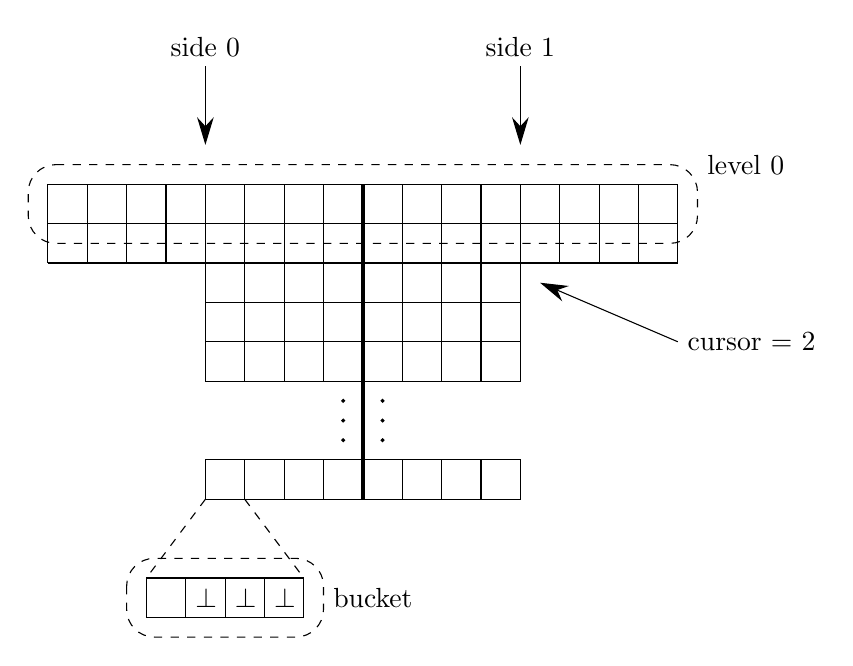
\begin{tikzpicture}
\draw (0,0) -- (8,0);
\draw (0,-0.5) -- (8,-0.5);
\draw (0,-1) -- (8,-1);

\draw (0,0) -- (0,-1);
\draw (0.5,0) -- (0.5,-1);
\draw (1,0) -- (1,-1);
\draw (1.5,0) -- (1.5,-1);
\draw (6.5,0) -- (6.5,-1);
\draw (7,0) -- (7,-1);
\draw (7.5,0) -- (7.5,-1);
\draw (8,0) -- (8,-1);

\draw (2,0) rectangle (6,-2);
\draw (2.5,0) rectangle (5.5,-2);
\draw (3,0) rectangle (5,-2);
\draw (3.5,0) rectangle (4.5,-2);

\draw (2,-1.5) -- (6,-1.5);
\draw (2,-2) -- (6,-2);
\draw[ultra thick] (4,0) -- (4,-4);

\draw[thin] (2,-3.5) rectangle (6, -4);
\draw (2.5,-3.5) rectangle (5.5, -4);
\draw (3,-3.5) rectangle (5, -4);
\draw (3.5,-3.5) rectangle (4.5, -4);

\draw (2, -2) rectangle (6, -2.5);
\draw (2.5, -2) rectangle (5.5, -2.5);
\draw (3, -2) rectangle (5, -2.5);
\draw (3.5, -2) rectangle (4.5, -2.5);

\filldraw (3.75,-2.75) circle (0.5pt);
\filldraw (3.75,-3) circle (0.5pt);
\filldraw (3.75,-3.25) circle (0.5pt);

\filldraw (4.25,-2.75) circle (0.5pt);
\filldraw (4.25,-3) circle (0.5pt);
\filldraw (4.25,-3.25) circle (0.5pt);

\draw [-{Stealth[length=10, width=6]}] (8,-2) -- (6.25,-1.25);
\draw (8,-2) node[right] {cursor = 2};

%\draw (4,-0.25) circle [x radius = 5.5, y radius = 0.375];
\draw (8.25,0.25) node[right] {level 0};

\draw[dashed, rounded corners=10] (-0.25,0.25) -- (8.25,0.25) -- (8.25,-0.75) -- (-0.25, -0.75) -- cycle;

\draw [-{Stealth[length=10, width=6]}] (2,1.5) -- (2,0.5);
\draw (2,1.75) node {side 0};
\draw [-{Stealth[length=10, width=6]}] (6,1.5) -- (6,0.5);
\draw (6,1.75) node {side 1};

\draw (1.25,-5) rectangle (3.25,-5.5);
\draw (1.75,-5) rectangle (2.75,-5.5);
\draw (2.25,-5) -- (2.25,-5.5);
\draw[dashed] (2,-4) -- (1.25,-5);
\draw[dashed] (2.5,-4) -- (3.25,-5);
\draw[dashed, rounded corners=10] (1,-4.75) rectangle (3.5,-5.75);
\draw (3.5, -5.25) node[right] {bucket};

\draw (1.75, -5.25) node[right] {$\bot$};
\draw (2.25, -5.25) node[right] {$\bot$};
\draw (2.75, -5.25) node[right] {$\bot$};

\end{tikzpicture}




\end{document}
